%% bare_jrnl.tex
%% V1.4b

\documentclass[journal]{IEEEtran}
\usepackage{svg}
\usepackage{graphicx}

\usepackage{listings}
\usepackage{xcolor}

% 定义 JSON 样式
\colorlet{punct}{red!60!black}
\definecolor{background}{HTML}{F8F8F8}
\definecolor{delim}{RGB}{20,105,176}
\colorlet{numb}{magenta!60!black}

\lstdefinelanguage{json}{ basicstyle=\normalfont\ttfamily, numbers=left,
numberstyle=\scriptsize, stepnumber=1, numbersep=8pt, showstringspaces=false,
breaklines=true, frame=lines, backgroundcolor=
\color{background}
, literate= *{0}{{{\color{numb}0}}}{1} {1}{{{\color{numb}1}}}{1} {2}{{{\color{numb}2}}}{1}
{3}{{{\color{numb}3}}}{1} {4}{{{\color{numb}4}}}{1} {5}{{{\color{numb}5}}}{1} {6}{{{\color{numb}6}}}{1}
{7}{{{\color{numb}7}}}{1} {8}{{{\color{numb}8}}}{1} {9}{{{\color{numb}9}}}{1} {:}{{{\color{punct}{:}}}}{1}
{,}{{{\color{punct}{,}}}}{1} {\{}{{{\color{delim}{\{}}}}{1} {\}}{{{\color{delim}{\}}}}}{1}
{[}{{{\color{delim}{[}}}}{1} {]}{{{\color{delim}{]}}}}{1}, }

\newcommand{\zz}[1]{{\color{red}ZZ: #1}}
\newcommand{\todo}[1]{{\color{red}TODO: #1}}


\usepackage{graphicx}
\usepackage{amsmath}
\usepackage{amssymb}
\usepackage{booktabs}
\usepackage{url}

% --- 核心修改：添加引用跳转支持 ---
\usepackage[colorlinks=true, linkcolor=black, citecolor=blue, urlcolor=blue]{
  hyperref
}

\hyphenation{op-tical net-works semi-conduc-tor}

\begin{document}
\title{Graph-Guided Long-Horizon Robotic Assembly via Vision-Language Reasoning and Logic-Geometric Programming}
% \title{Image-to-Assembly: Autonomous Robotic Assembly via Vision-Language Reasoning and Logic-Geometric Programming}

\author{Anonymous Authors}
 % <-this % stops a space
%\thanks{This paper was produced by the IEEE Publication Technology Group. They are in Piscataway, NJ.}% <-this % stops a space
%\thanks{Manuscript received April 19, 2021; revised August 16, 2021.}

\markboth{IEEE Robotics and Automation Letters}%
{Anonymous Authors: Image-to-Assembly: Autonomous Robotic Assembly via Vision-Language Reasoning and Logic-Geometric Programming}

\maketitle

\begin{abstract}
Autonomous robotic assembly is a fundamental capability for flexible and adaptive manufacturing.
Yet, it remains challenging to derive executable long-horizon plans from visual task specifications, while satisfying both geometric and physical constraints in unstructured scenes.
This letter presents a framework for planning robotic structural assembly from a target image in unstructured scenes.
Instead of using a vision language model (VLM) to directly generate precise geometry or executable robot actions, our proposed method used the VLM to infer an object support graph, describing the structural dependencies of the targeted assembly. A two-level graph decomposition partitions the resulting long-horizon task into precedence-consistent and solver-manageable batches.
For each batch, scene grounding filters candidate object instances according to geometric reachability and ranks feasible alternatives according to manipulability.
The grounded batch is then solved using selective logic geometric programming (LGP), with collision constraints instantiated for geometrically relevant object pairs, and executed iteratively on a physical robot.

Experiments ...[TODO] add experimental results

Our experimental results demonstrate the potential of structured VLM reasoning to improve the scalability of geometrically constrained, long-horizon robotic assembly.
\end{abstract}

\begin{IEEEkeywords}
Robotic Assembly, Vision-Language Model, Logic-Geometric Programming, Task and Motion Planning
\end{IEEEkeywords}

\section{Introduction}

Long-horizon multi-part robotic assembly is a fundamental capability for intelligent manufacturing and embodied robotics, with broad applications in both industrial production and daily household environments. 
Unlike single-step manipulation, these tasks require the robot to accomplish a sequence of interdependent assembly operations while satisfying task dependencies and physical constraints. 
Automating such processes could greatly expand the practical deployment of robotic assembly systems by reducing manual programming effort and improving adaptability to diverse tasks. 
However, achieving autonomous long-horizon assembly remains challenging, as the robot must accurately infer the assembly objective, generate a logically consistent task plan, and produce physically feasible motions for each assembly step. 
Moreover, the tight coupling between high-level task planning and low-level motion planning, together with the long-term dependencies across assembly decisions, further increases the complexity of reliable autonomous assembly.

Classical approaches to long-horizon robotic assembly are primarily built on model-based Task and Motion Planning (TAMP), which typically employs symbolic planners, such as those based on Planning Domain Definition Language (PDDL), to generate task plans, followed by motion planners to compute feasible trajectories for each action.
A representative TAMP approach is Logic-Geometric Programming (LGP), which integrates task planning and motion planning into a unified optimization framework, allowing motion feasibility to be considered during task planning rather than as a separate step.
By explicitly modeling task semantics and constraints, these methods produce interpretable and verifiable planning results. 
However, they heavily rely on manually specified task definitions, object models, and action rules, requiring substantial engineering effort and domain expertise. 
Consequently, extending these methods to new objects or assembly objectives often needs manual redesign of symbolic models and planning rules, limiting their scalability and adaptability to diverse real-world scenarios.

Recently, Large Language Models (LLMs) have been introduced to robotic assembly to improve high-level task understanding and planning. 
By leveraging their reasoning capabilities, LLMs are able to directly interpret human instructions, infer assembly intent, and generate task plans without manually defined symbolic specifications. 
This capability greatly reduces engineering effort and improves adaptability to diverse tasks, thereby enabling more flexible robotic assembly systems in changing environments. 
However, the generated task plans are not guaranteed to be logically correct or physically executable, as LLMs lack reliable reasoning over kinematic constraints and motion feasibility. 
Another practical limitation is that most existing LLM-based approaches assume natural language instructions as input, whereas many real-world assembly tasks, particularly in industrial settings, are specified by target assembly images rather than textual descriptions.

In this work, we aim to realize autonomous long-horizon robotic assembly directly from a target assembly image while ensuring safe and reliable motion execution. 
To this end, we propose a unified framework that combines the visual reasoning capability of Vision-Language Models (VLMs) with the optimization-based guarantees of LGP. 
Given a target assembly image and the current scene, the framework infers the assembly goal, identifies the required object components, determines an appropriate assembly sequence, and generates executable robot motions that satisfy kinematic and dynamic constraints. 
Specifically, it consists of three key components: 
(1) \textit{VLM-Based Task Understanding}: the VLM first interprets the target assembly image to construct an assembly graph, from which assembly action plans are derived through graph decomposition and clustering; 
(2) \textit{Reachability-Manipulability-Aware Scene Understanding}: the robot then perceives the workspace, identifies the corresponding manipulatable objects, and prioritizes them according to reachability and manipulability; 
(3) \textit{LGP-Based Motion Execution}: finally, the derived task plan and scene information are integrated into an LGP to produce collision-free and physically feasible motion trajectories for completing the assembly task. 
Note that, the computational complexity of LGP increases rapidly with the number of objects, making its direct usage in long-horizon assembly problems impractical. 
To address this issue, we decompose the overall assembly process into a sequence of short-horizon subtasks during the VLM-based task understanding, and introduce an active-constraint LGP formulation to further improve computational efficiency.



\todo{add experiments and results descriptions} 
We evaluate our methods on... 
The results show that...

\todo{add contributions}
Our main contributions are threefold:
\begin{itemize}
    \item A constrained VLM interface for extracting an assembly representation from a target image;
    \item A formal, precedence-preserving decomposition that produces solver-bounded LGP subproblems;
    \item An end-to-end evaluation of graph quality, planning scalability, and physical execution.
\end{itemize}


\section{Related Work}

\todo{Write reference section, about 0.8 page, no more than 1 page}
\subsection{Assembly Sequence Planning and Structural Representations}

Assembly Sequence Planning (ASP) is typically defined as the process of transforming the final target structure into a series of executable component assembly operations.
Classic ASP research typically employs graph structures to represent feasible assembly sequences, constraint relationships, and sub-assembly states.
Typical methods include precedence graphs, contact graphs, support graphs, and AND/OR graphs.
There are also graph decomposition methods for construction and stacking tasks.
The priority graph is typically used to represent sequential constraints between different assembly operations.
The contact graph and connection graph are used to describe physical contact, connection, or interference relationships between parts.
The support graph further considers factors such as gravity, load-bearing capacity, and the stability of intermediate structures.
The AND/OR graph decomposes assembly tasks into multiple intermediate structures, thereby reducing search complexity.
For building construction and block-stacking tasks, the graph decomposition method is often combined with stability constraints to ensure that the intermediate structures generated at each step are physically feasible.

In recent years, the input formats for assembly tasks have expanded from traditional CAD models to include images, instruction manuals, and multi-modal instructions.
However, most methods still rely on known geometric models, predefined part relationships, manually designed support relationships, or assembly instructions that already contain step information.
In other words, existing methods typically assume that assembly relationships are already given, rather than deriving usable structures directly from visual information.
Unlike these methods, the system proposed in this paper extracts a structured representation from target images for LGP solving.
LGP transforms the target assembly state in the image into an input containing symbolic relationships and geometric constraints.
This bridges the gap between visual task descriptions and executable autonomous assembly planning.

\subsection{Task and Motion Planning for Long-Horizon Assembly}
Long-horizon assembly tasks can typically be modeled as Task and Motion Planning (TAMP) problems, in which discrete assembly decisions and continuous robot motion must be considered together.
In integrated TAMP frameworks such as LGP, symbolic task selection and geometric motion constraints are solved through a unified optimization process.
LGP is a typical TAMP formulation method that combines discrete logic programming with continuous trajectory optimization.
Since the feasibility of assembly operations depends not only on logical order but is also influenced by constraints such as reachability, stability, and contact relationships, LGP is suitable for describing complex assembly tasks.
However, when assembly tasks involve multiple objects and long sequences of operations, directly solving the LGP problem leads to a rapid expansion of the search space.

To improve the scalability of long-horizon LGP, existing research typically employs methods such as hierarchical LGP, receding-horizon LGP, heuristic search, and subproblem decomposition.
These methods can reduce the scale of a single solution.
However, fixed-horizon may overlook object dependencies and support relationships within the assembly.
And the receding-horizon method may lack global structural information and require frequent re-planning.
The decomposition method proposed in this paper is not based on the fixed-horizon but rather divides the task according to the assembly structure inferred from the target image.
By extracting object relationships, support dependencies, and sub-assemblies, this structural information is defined as individual LGP subproblems.
The method proposed in this paper preserves the global assembly intent while keeping the subproblems simple.

\subsection{Foundation Models in Robotic Assembly}
Foundational models have been widely adopted in robotic manipulation and assembly tasks to enhance task understanding and long-term planning capabilities.
Some studies utilize Large Language Models (LLM) to generate high-level task plans based on natural language instructions.
Other studies utilize Visual-Language Models (VLM) to identify objects in images, infer spatial relationships, and generate assembly steps.
Furthermore, Visual-Language-Action (VLA) models attempt to directly map visual observations and language instructions to robotic actions, thereby enabling end-to-end manipulation control.
While these methods enhance task understanding and action generation, they lack an explicit representation of geometric feasibility, contact constraints, support dependencies, and stability conditions in long-term assembly tasks.

To improve reliability, many studies adopt modular systems that combine LLM/VLM with classical planners, linking perception and planning through scene graphs, object relationships, and constraints.
Compared to free-form text, this type of structured output is better suited for robotic execution.
However, most existing methods are designed for general scene understanding and are not specifically optimized for tasks and motion planners based on LGP.
The VLM proposed in this paper outputs a constrained representation of assembly relationships, extracting information directly from target images.
And converts it into input for LGP.
Therefore, this paper does not directly generate actions using the VLM.
This paper uses the VLM to establish an interface between visual target descriptions and LGP long-time-domain assembly planning.


\subsection{Assembly Sequence Planning and Structural Representations}

Topics to cover (follow the sequence of autonomous assembly, cover them one by one):
- precedence graphs
- contact and support graphs
- subassembly generation
- assembly ordering, which also covers stability constraints/considerations
- graph decomposition for construction and stacking
- assembly specified by image, CAD, instruction, etc.

The review of literature should converge to the message i.e. existing structural representations generally assume a known geometric model or predefined relations; our proposed system derives a solver-oriented (i.e., LGP) structure from a target image.

\subsection{Task and Motion Planning for Long-Horizon Assembly}

Cover in this subsection:

- integrated TAMP
- LGP and KOMO
- receding-horizon or hierarchical LGP
- heuristic search reduction
- reachability-guided planning
- subproblem decomposition in construction and assembly

The comparison with literature must clarify how the proposed decomposition differs from: (1) generic fixed-horizon, or (2) receding-horizon approaches.

\subsection{Foundation Models in Robotic Assembly}

Cover:
- LLM-generated plans
- VLM-based scene + task reasoning
- direct visuomotor or VLA methods
- modular systems, e.g., VLM + planner
- structured outputs, e.g., scene graphs, constraints, and sub-goals

This review should point out the gap in the literature:
our proposed VLM produces a constrained assembly relation representation specifically designed for downstream LGP


\section{Problem Formulation}
\label{sec:problem_formulation}

\todo{Move the problem statement into here: please formulating it using mathematical definitions, e.g., what is the input, what is the output, which variables/components are processed}

\todo{Write something like: first we have an image $\mathcal{I}$ as the input, we need to determine the assembly goal $\mathcal{G}$ from this image. Then, this goal $\mathcal{G}$ should also be used to determine the task plan $\mathcal{P}$, and how to associate the $\mathcal{G}$ and $\mathcal{P}$ with the current scene, determining objects to be manipulated, how to determining motions, etc.}

\todo{Note that: problem formulation is not about details of your method, it is about \textbf{what is your PROBLEM, and how is this problem defined by math}!}

We consider the problem of planning a long-horizon robotic assembly directly
from a target assembly image, without assuming a predefined object model or
symbolic task specification. The input to the system is a target assembly
image $\mathcal{I}$, together with the current physical scene
$\mathcal{S}=\{o_1,\dots,o_N\}$, where each $o_i$ denotes an object instance
characterized by its pose and geometric attributes.

The first problem is to determine the assembly goal from $\mathcal{I}$. We
represent this goal as an object-support graph $\mathcal{G}=(\mathcal{V},\mathcal{E})$,
where each node $v\in\mathcal{V}$ denotes one target object instance and each
directed edge $(u,v)\in\mathcal{E}$ denotes that object $u$ must support
object $v$ in the completed assembly:
\begin{equation}
  \mathcal{G} = f_{\mathrm{VLM}}(\mathcal{I}).
  \label{eq:problem_goal}
\end{equation}

The second problem is to determine a task plan $\mathcal{P}$ for realizing
$\mathcal{G}$. We represent $\mathcal{P}=(B_1,\dots,B_M)$ as an ordered
sequence of $M$ execution batches, in which every node of $\mathcal{V}$
appears in exactly one batch, each batch respects a solver-imposed size
bound, and every node in $B_m$ has all of its supporters already placed in an
earlier batch $B_1,\dots,B_{m-1}$:
\begin{equation}
  \mathcal{P} = f_{\mathrm{decomp}}(\mathcal{G}).
  \label{eq:problem_plan}
\end{equation}

The third problem is to associate $\mathcal{G}$ and $\mathcal{P}$ with the
current scene $\mathcal{S}$, i.e., to determine which concrete object
instance should be used to realize each node $v\in\mathcal{V}$. This requires
a grounding map $\pi:\mathcal{V}\to\mathcal{S}_{\mathrm{feas}}$, where
$\mathcal{S}_{\mathrm{feas}}\subseteq\mathcal{S}$ is the subset of instances
that are kinematically reachable, and $\pi$ additionally prefers instances
that are easier for the robot to manipulate.

Finally, for each grounded batch $\pi(B_m)$, the system must determine a
collision-free, physically feasible motion trajectory $x_m^\ast$ that
realizes the corresponding support relations under the kinematic and dynamic
constraints of the robot. The overall problem is therefore to find
\begin{equation}
  \mathcal{G},\quad \mathcal{P},\quad \pi,\quad \{x_m^\ast\}_{m=1}^{M}
  \label{eq:problem_all}
\end{equation}
such that executing $\{x_m^\ast\}_{m=1}^{M}$ on the physical robot yields a
final scene configuration consistent with the support relations specified by
$\mathcal{G}$.


\section{Method}


This section presents the proposed framework for accomplishing long-horizon robotic assembly from a target assembly image. 
As illustrated in Fig.~\ref{fig:workflow}, the framework consists of three components. 
First, a VLM analyzes the target assembly image to construct an assembly graph and generate a sequence of assembly actions (Sec.~\ref{sec:task_understanding}). 
Second, the robot perceives the workspace to identify the corresponding objects and prioritize them according to reachability and manipulability (Sec.~\ref{sec:scene_understanding}). 
Finally, the task plan and scene information are integrated into a LGP formulation to produce feasible motions for each assembly step (Sec.~\ref{sec:motion_execution}). 

\todo{write the method corresponding to the outline given in the last paragraph of the introduction, we have three components, detail each one in one subsection}

\subsection{VLM-Based Task Understanding}
\label{sec:task_understanding}

\todo{Introduce in each subsubsection: 1. how VLM converts the image input into assembly graph. 2. How this graph is converted into action plans}

\subsubsection{VLM for Assembly Graph Generation}
\textcolor{red}{Input: Image, Output: Graph}

Following the mapping $\mathcal{G}=f_{\mathrm{VLM}}(\mathcal{I})$ introduced in
Section~\ref{sec:problem_formulation}, we use a VLM to convert the target
assembly image $\mathcal{I}$ into the object-support graph
$\mathcal{G}=(\mathcal{V},\mathcal{E})$, rather than asking it to predict
precise object coordinates or a long executable program directly. This
choice follows the capability boundary of current VLMs: they are
comparatively reliable at inferring relational structure, support
dependencies, and coarse left-right or above-below organization, but less
stable when required to output exact geometry, long symbolic code, or
mathematically precise layouts. We therefore let the VLM produce the
structural representation that it is best suited to provide. Each node
$v \in \mathcal{V}$ denotes one target object instance, and each directed
edge $(u,v) \in \mathcal{E}$ indicates that object $u$ must support object
$v$ in the final assembly. The graph is directed because support precedence
is asymmetric, and optional local labels such as left/right placement hints
are retained only as geometric side information rather than as the
execution order itself.

\subsubsection{Graph Decomposition and Clustering}
\textcolor{red}{Input: Graph, Output: Short-horizon action plans}

Following the mapping $\mathcal{P}=f_{\mathrm{decomp}}(\mathcal{G})$
introduced in Section~\ref{sec:problem_formulation}, this step converts the
support graph $\mathcal{G}$ into the task plan
$\mathcal{P}=(B_1,\dots,B_M)$, i.e., a precedence-consistent sequence of
short-horizon execution batches. Exposing the full graph to the solver at
once is impractical, whereas placing objects strictly one at a time is
unnecessarily slow; the decomposition must also respect support precedence,
so that no object is scheduled before all of its supporters. We therefore
compute $f_{\mathrm{decomp}}$ in two stages that operate directly on
$\mathcal{G}$: a coarse branch grouping followed by a per-branch cutting
into solver-sized batches.

The first stage, \emph{branch-based grouping}, identifies the coarse
structural organization of $\mathcal{G}$. We assign each node $v$ a layer
number by propagating outward from the table root, which is fixed to
layer~$0$:
\begin{equation}
  \mathrm{layer}(v) =
  \begin{cases}
    0, & \mathrm{supporters}(v)=\varnothing,\\[2pt]
    1 + \displaystyle\max_{u \in \mathrm{supporters}(v)} \mathrm{layer}(u), & \text{otherwise,}
  \end{cases}
  \label{eq:layer}
\end{equation}
where $\mathrm{supporters}(v)$ is the set of nodes with a direct edge into
$v$; only the table root has no supporters, so every object resting on the
table has layer~$1$. Each layer-$1$ node is assigned to a branch according
to the placement label (e.g., left/right) of its table support, and this
branch label is propagated to higher layers along the support edges; a node
whose supporters belong to two or more distinct branches is instead assigned
to a dedicated \emph{bridge} branch. This stage groups $\mathcal{V}$ into a
small number of branches without yet committing to an execution order.

The second stage, \emph{layer-based cutting}, turns the grouped graph into
the ordered batch sequence $\mathcal{P}$. The branches are first ordered so
that a branch is cut only after every branch it depends on, through
cross-branch support edges, has already been scheduled. Each branch is then
cut independently: its nodes are processed in increasing support depth, and
at each depth the nodes sharing the same in-branch supporter set
\begin{equation}
  r(v) = \{\, u \in \mathrm{supporters}(v) : \mathrm{branch}(u)=\mathrm{branch}(v) \,\}
  \label{eq:role}
\end{equation}
are collected, ordered by node identifier for a deterministic result, and
split into batches of at most $B_{\max}=2$ nodes. Concatenating the batches
of all branches in order yields $\mathcal{P}$. For a nine-object assembly
with three independent branches (objects $1,3,4$; $2,5,6$; $7,8,9$), this
procedure yields
\begin{equation}
  \mathcal{P} = \big(\{1\},\{3,4\},\{2\},\{5,6\},\{7\},\{8\},\{9\}\big),
  \label{eq:plan_example}
\end{equation}
where each set is one execution batch $B_m$ submitted to the solver. The
batch bound $B_{\max}=2$ reflects the scale at which the downstream solver
remains efficient under our hardware constraints.

\subsection{Reachability-Manipulability-Aware Scene Understanding}
\label{sec:scene_understanding}

\todo{Introduce in each subsubsection: 1. how reachability is considered. 2. How manipulability is used to order the list of the manipulable objects}

\subsubsection{Reachability Filtering}
\textcolor{red}{Input: Scene Information, Output: Reachability filtered list of objects}

This step takes the current scene $\mathcal{S}=\{o_1,\dots,o_N\}$ introduced
in Section~\ref{sec:problem_formulation} and returns the subset
$\mathcal{S}_{\mathrm{feas}}\subseteq\mathcal{S}$ of object instances that
the robot can actually reach. We apply two successive filters: a cheap
geometric prior that discards obviously inaccessible objects, followed by a
rigorous kinematic check on the survivors.

The first filter assigns each object a scalar geometric score $\rho(o_i)$
based on its position relative to the surrounding scene geometry, combining a
density term $\rho_{\mathrm{gmm}}$ and a clearance term $\rho_{\mathrm{esdf}}$.
The density term is a Gaussian kernel of bandwidth $\sigma = 0.12\,\mathrm{m}$
evaluated over the pick points of all objects in $\mathcal{S}$:
\begin{equation}
  \rho_{\mathrm{gmm}}(o_i) = \frac{1}{N} \sum_{j=1}^{N}
    \exp\!\left(-\frac{\|p_i - p_j\|^2}{2\sigma^2}\right),
  \label{eq:reach_gmm}
\end{equation}
where $p_i$ is the pick point of object $o_i$ (the handle sub-frame center
if available, otherwise the geometric center), and a higher value indicates
that $o_i$ lies in a geometrically central, more accessible region. The
clearance term measures the distance to surrounding obstacles, each
approximated as a bounding sphere with center $c_k$ and radius $r_k$:
\begin{equation}
  \rho_{\mathrm{esdf}}(o_i) = \min_k \frac{\max\!\left(0,\ \min\!\left(\|p_i - c_k\| - r_k,\ d_{\max}\right)\right)}{d_{\max}},
  \label{eq:reach_esdf}
\end{equation}
with $d_{\max} = 0.20\,\mathrm{m}$, so that a higher value indicates more
open space around the object. The two terms are linearly combined into the
geometric score,
\begin{equation}
  \rho(o_i) = \alpha \, \rho_{\mathrm{gmm}}(o_i) + \beta \, \rho_{\mathrm{esdf}}(o_i),
  \qquad \alpha = 0.6,\ \beta = 0.4,
  \label{eq:reach_fused}
\end{equation}
and an object passes this filter if $\rho(o_i) \geq \tau_r = 0.45$.

The second filter verifies kinematic feasibility on the objects that survive
the geometric prior. For each such candidate $o_i$, we construct a
single-step KOMO subproblem $\Pi_i^{\mathrm{pick}}$ that asks the solver to
find a robot configuration from which a grasp of $o_i$ can be initiated,
using the same KOMO/RAI framework and the full set of kinematic and
collision constraints as the main solver. The object is retained only if
this subproblem is feasible:
\begin{equation}
  \mathrm{Reach}(o_i) =
  \mathbb{I}\!\left[\mathrm{Feasible}\!\left(\Pi_i^{\mathrm{pick}}(o_i)\right)\right].
  \label{eq:reach_check}
\end{equation}
The two filters are complementary: the geometric prior removes clearly
unreachable objects at negligible cost, while the pick-waypoint check
provides rigorous verification only where it is needed. The output is the
reachable subset
$\mathcal{S}_{\mathrm{feas}} = \{\, o_i \in \mathcal{S} : \rho(o_i)\ge\tau_r \ \wedge\ \mathrm{Reach}(o_i)=1 \,\}$,
which is passed to the ordering step below.

\begin{figure*}[!t]
  \centering
  
\includegraphics[width=\textwidth]{Reachability.png}
  \caption{Reachability screening result: objects passing both the geometric prior and the pick-waypoint feasibility check are retained, while remaining candidates are pruned before downstream LGP solving.}
  \label{fig:reachability}
\end{figure*}

\subsubsection{Manipulability-Aware Object Ordering}
\textcolor{red}{Input: Reachability filtered list of object, Output: Manipulability ordered list of objects}

This step takes the reachable subset $\mathcal{S}_{\mathrm{feas}}$ and
orders its instances by how comfortably the robot arm can approach them, so
that the grounding map $\pi$ of Section~\ref{sec:problem_formulation} can
prefer easier-to-manipulate instances. For each object
$o_i \in \mathcal{S}_{\mathrm{feas}}$, we define an approach target slightly
above the object, solve a damped least-squares inverse kinematics problem
for that target, and evaluate the positional Yoshikawa manipulability score
at the resulting configuration $q_i$:
\begin{equation}
  m(o_i) = \sqrt{\det\!\left(J_p(q_i)\,J_p(q_i)^\top\right)},
  \label{eq:manip}
\end{equation}
where $J_p(q_i)$ is the position Jacobian of the robot at $q_i$. A higher
$m(o_i)$ indicates a more dexterous approach configuration. Within each
object category, instances are ranked by decreasing $m(o_i)$, and instances
whose inverse kinematics fails are placed last. The output is thus, for each
category, a manipulability-ordered list of reachable instances; this
ordering defines the preference that the grounding map $\pi$ uses to select
a concrete instance when a batch requires an object of that category.

\begin{figure*}[!t]
  \centering
  \setlength{\tabcolsep}{2pt}
  \begin{tabular}{@{}cccc@{}}
    
\includegraphics[width=0.24\textwidth]{Manipulability_1.png} &
    
\includegraphics[width=0.24\textwidth]{Manipulability_2.png} &
    
\includegraphics[width=0.24\textwidth]{Manipulability_3.png} &
    
\includegraphics[width=0.24\textwidth]{Manipulability_4.png} \\
    \small (a) & \small (b) & \small (c) & \small (d)
  \end{tabular}
  \caption{Manipulability scores for four candidate object instances: (a) 3D manipulability field, (b)--(d) orthogonal slices. Higher scores indicate more dexterous approach configurations; instances are ranked accordingly for scene-side grounding.}
  \label{fig:manipulability}
\end{figure*}

\subsection{LGP-Based Motion Execution}
\label{sec:motion_execution}

\todo{Introduce in each subsubsection: 1. how LGP is used to solve the motion with active constraints. 2. how motion trajectories are executed on the robot}

Sections~\ref{sec:task_understanding} and~\ref{sec:scene_understanding}
produce two parallel results that must be combined before solving: the task
plan $\mathcal{P}=(B_1,\dots,B_M)$, whose batches specify the structural
slots to be filled (e.g., placing a box-type object on top of an existing
one), and, for each object category, a reachable and manipulability-ordered
list of concrete scene instances. The grounding map $\pi$ of
Section~\ref{sec:problem_formulation} merges the two streams: each structural
slot in the current batch $B_m$ is bound to a concrete instance by scanning
down the ranked candidate list for the required category until a feasible
match is found. This produces a fully grounded batch $\pi(B_m)$, i.e., a list
of concrete object-to-role assignments, which is the input handed to the
solver.

\subsubsection{LGP with Active Constraints}
\textcolor{red}{Input: Action Plans and List of Objects, Output: LGP optimization with active constraints for finding motion trajectories}

Native LGP couples symbolic task structure with continuous trajectory
optimization through a shared representation of predicates, action semantics,
and decision rules~\cite{cite_lgp_2015}. In principle this abstraction can
solve an assembly task from a symbolic goal alone, but in long-horizon
settings exposing the full generic task domain leads to excessive symbolic
branching and unnecessary geometric backtracking. We therefore instantiate
the native LGP abstraction selectively for each grounded batch $\pi(B_m)$,
compiling only the symbolic relations, object bindings, and decision rules
required by the support pattern active in that batch. The solver thus
receives a grounded symbolic-geometric subproblem tailored to $B_m$ rather
than a monolithic domain covering all possible assembly alternatives.

Discretising a trajectory as $\mathbf{x}_{0:T}=\{x_0,x_1,\dots,x_T\}$ over
$T$ time steps, we keep the native LGP formulation in its original joint
form~\cite{cite_lgp_2015},
\begin{align}
\min_{\substack{x,\,a_{1:K},\\ s_{1:K},\,t_{1:K}}}\quad
&\int_0^T c\!\left(x(t),\dot{x}(t),\ddot{x}(t)\right)\,dt + \psi\!\left(x(T)\right)
\label{eq:lgp_obj}\\
\text{s.t.}\quad
&\forall k=1{:}K\ \ s_k = \mathrm{succ}(a_k, s_{k-1}),
\label{eq:lgp_succ}\\
&s_K\models g,
\label{eq:lgp_goal}\\
&\forall_{k=1}^{K}\ h_{\mathrm{switch}}\!\left(x(t_k)\mid a_k,s_{k-1}\right)=0,
\label{eq:lgp_sweq}\\
&\forall_{k=1}^{K}\ g_{\mathrm{switch}}\!\left(x(t_k)\mid a_k,s_{k-1}\right)\le 0,
\label{eq:lgp_swineq}\\
&\forall t\in[0,T]\ h_{\mathrm{path}}\!\left(x(t),\dot{x}(t)\mid s_{k(t)}\right)=0,
\label{eq:lgp_patheq}\\
&\forall t\in[0,T]\ g_{\mathrm{path}}\!\left(x(t),\dot{x}(t)\mid s_{k(t)}\right)\le 0,
\label{eq:lgp_pathineq}
\end{align}
where $a_{1:K}$, $s_{1:K}$, and $t_{1:K}$ are the action, symbolic-state, and
switch-time sequences, $g$ is the symbolic goal induced by batch $B_m$, and
$s_k=\mathrm{succ}(a_k,s_{k-1})$ encodes the logic transitions.

For each grounded batch we then solve the corresponding $k$-order Markov
Optimization (KOMO) subproblem in its original constrained sum-of-squares
form~\cite{cite_komo_2014}, i.e., the continuous trajectory-optimization
component of LGP, computing robot and object motions subject to kinematic,
task, and collision constraints:
\begin{align}
\min_{x_{0:T}}\quad
&\sum_{t=0}^{T} f_t\!\left(x_{t-k:t}\right)^\top f_t\!\left(x_{t-k:t}\right)
+\sum_{t,t'} k(t,t')\,x_t^\top x_{t'}
\label{eq:komo}\\
\text{s.t.}\quad
&\forall t:\ g_t\!\left(x_{t-k:t}\right)\le 0,\ h_t\!\left(x_{t-k:t}\right)=0.
\label{eq:komo_c}
\end{align}

The waypoint-level solve also supplies geometric cues that let the downstream
full-motion solve be selective about the collision constraints it
instantiates. Let $x$ denote the full-motion trajectory, $d_{ij}(x)$ the
minimum pairwise distance between collision proxy frames $f_i$ and $f_j$
along $x$, and $f_i^w$ the pose of frame $f_i$ at waypoint $w$. The
trajectory for batch $B_m$ is obtained as
\begin{equation}
x_m^\ast = \arg\min_x J(x),
\label{eq:act_obj}
\end{equation}
subject to collision constraints instantiated only for the active set,
\begin{equation}
c_{ij}(x) = d_{\mathrm{safe}} - d_{ij}(x) \leq 0,
\quad \forall (f_i, f_j) \in \mathcal{C}_{\mathrm{active}}(w),
\label{eq:act_c}
\end{equation}
\begin{equation}
\mathcal{C}_{\mathrm{active}}(w) =
\left\{(f_i, f_j)\ \middle|\ d(f_i^w, f_j^w) < r_{\mathrm{active}}\right\},
\label{eq:act_set}
\end{equation}
where $J(x)$ is the downstream motion objective, $d_{\mathrm{safe}}$ the
prescribed safety margin, and $r_{\mathrm{active}}$ the activation radius
used to screen candidate collision pairs from the waypoint geometry. Only
pairs in $\mathcal{C}_{\mathrm{active}}(w)$ become explicit collision
constraints in the full-motion solve, which reduces unnecessary collision
checks and shortens solve time without altering the structural plan. The
output of this step is the collision-free trajectory $x_m^\ast$ for the
current batch: the decomposition module decides which support relations to
realize next, and native LGP resolves whether and how they can be executed
under the current scene geometry.

\subsubsection{Motion Execution with Joint-Space Impedance Control}
\textcolor{red}{Input: motion trajectories, Output: impedance control for joint torques for motion execution}

Once the trajectory $x_m^\ast$ of a batch is obtained, it is parsed into a
joint-space trajectory and the associated gripper commands and dispatched to
the robot controller for execution on the physical platform. On our Franka
manipulator, the controller tracks the planned joint trajectory through the
arm's built-in joint-space impedance regulation, which converts the tracking
error into joint torques and yields compliant, safe execution at the torque
level; this control layer is a standard property of the platform rather than
a component optimized in this work. The execution layer itself remains
intentionally thin: it streams the planned motion and gripper switches to the
robot and updates the scene state for the next planning--solving cycle, after
which the pipeline proceeds to the following batch $B_{m+1}$.


\section{Results}

\subsection{Experimental Setup and Evaluation Design}
\label{subsec:setup}

We evaluate the proposed framework on a Franka Emika Panda manipulator, with
all planning performed through the RAI/KOMO solver. For reasons of hardware
limitation and solving efficiency, we cap the memory available to each planning
task at $16$\,GB, and all reported numbers are obtained under this limit.

We consider two task families chosen to probe complementary capabilities.
\emph{Cube-stacking} assemblies, ranging from four to eight cubes, assess the
ability to handle \emph{long-horizon} construction, where the number of
interdependent placement steps grows with the structure. Assemblies from the Functional Manipulation Benchmark (FMB),
ranging from three to five objects, assess \emph{fine-grained, logically
constrained} assembly, where objects must be inserted precisely and in a strict
support order; we adapt the benchmark's objects, adjusting their dimensions and
shapes, to match our manipulator's workspace and the geometry of our assembly
tasks. For each task we further distinguish two scene conditions: a
no-redundancy setting (NR), in which the scene contains exactly the objects
required by the target, and a redundancy setting (R), in which additional
distractor objects of the same types are present, so that the system must first
identify the correct instances before planning.

We compare three methods. \emph{Direct-Action LLM} queries a VLM to output
executable pick-and-place waypoints directly from the target image, without any
intermediate structural representation. \emph{Global LGP} is the native LGP
baseline that solves each assembly as a single monolithic problem, without
decomposition. \emph{Smart} is our proposed method, which combines the
two-level graph decomposition of Section~\ref{sec:task_understanding} with the
selective, active-constraint LGP solving of Section~\ref{sec:motion_execution}.
Our evaluation proceeds in three stages: we first show that the Direct-Action
LLM baseline cannot produce executable motions
(Section~\ref{subsec:res_direct}); we then compare Smart against Global LGP on
long-horizon stacking (Section~\ref{subsec:res_scal}) and on fine-grained FMB
assembly (Section~\ref{subsec:res_fmb}); and we finally report physical
execution on the real robot (Section~\ref{subsec:res_real}).

We report planning success rate, solving time over successful trials, and
physical execution outcomes. For both task families, a configuration is one
(magnitude, method, condition) triple, and the evaluation is designed so that
each configuration is run for $50$ trials, drawn from five scene scenarios each
instantiated with ten random seeds.

\subsection{Direct-Action LLM Baseline is Infeasible}
\label{subsec:res_direct}

We first examine whether a VLM can plan assembly directly, without the
structural interface introduced in this work. In the Direct-Action LLM
baseline, the VLM receives the target image together with the scene description
and is asked to emit, for every object, the complete pick-and-place motion as a
sequence of end-effector waypoints and gripper events.

This baseline consistently fails to produce executable assemblies. Although the
VLM reliably returns syntactically valid waypoint sequences, the numerical poses
it generates are geometrically inconsistent: grasp points miss the target
objects, intermediate waypoints penetrate the table or previously placed
structure, and placement heights violate the support order. Representative
failures are shown in the supplementary video. This behavior confirms the
capability boundary discussed in Section~\ref{sec:task_understanding}: current
VLMs are unreliable when required to output exact geometry and long, metrically
precise action sequences.

The same models, however, are far more dependable at inferring relational
structure. This contrast is the central motivation of our design: instead of
asking the VLM for precise motions, we use it only to produce the
object-support graph, and delegate all metric and collision reasoning to LGP.
The remaining experiments evaluate this division of labor.

\subsection{Scalability on Long-Horizon Stacking}
\label{subsec:res_scal}

\begin{figure*}[!t]
\centering

\includegraphics[width=\textwidth, height=0.40\textheight, keepaspectratio]{Cube_Stacking.png}
\caption{Representative cube-stacking task setup. Assemblies ranging from four to eight cubes are used to evaluate long-horizon planning scalability.}
\label{fig:cube_stacking}
\end{figure*}

We next compare Smart against the Global LGP baseline on cube-stacking
assemblies of increasing size, which directly probes long-horizon scalability.
Table~\ref{tab:cube_sr} reports planning success rate and
Table~\ref{tab:cube_time} the average solving time over successful trials.

Smart solves every configuration: it attains a $100\%$ success rate for all
magnitudes from four to eight cubes, under both the no-redundancy (NR) and
redundancy (R) conditions. Global LGP, in contrast, degrades as the assembly
grows, and the effect is most severe under redundancy. Without redundancy,
Global remains close to fully reliable up to seven cubes ($93.3$--$100\%$) and
drops to $60\%$ only at eight cubes; with redundancy it degrades much earlier,
falling to $56$--$57\%$ by five to six cubes and collapsing to $3.7\%$ at seven
cubes and to $0\%$ at eight cubes, where the monolithic search must
disambiguate distractor objects while jointly optimizing the full-horizon
trajectory.

The solving-time comparison shows the same trend from the efficiency side.
Smart keeps solving time low and slowly growing, from about $29$\,s at four
cubes to $55$\,s at eight cubes. Global LGP instead scales poorly under
redundancy: its solving time rises to $146$\,s at six cubes and $296$\,s at
seven cubes, an order of magnitude above Smart at the same size. The eight-cube
R entry for Global is reported as zero solving time because no trial succeeded.

Exposing only a solver-manageable batch at
each step, rather than the full monolithic problem, is what makes long-horizon
assembly tractable: Smart preserves both reliability and efficiency as the
horizon grows, whereas the native LGP baseline becomes unreliable and, when it
does succeed, dramatically slower.

\begin{table}[!t]
\centering
\caption{Cube-stacking planning success rate (\%): Smart (ours) vs Global LGP,
under no-redundancy (NR) and redundancy (R) conditions.}
\label{tab:cube_sr}
\begin{tabular}{lcccc}
\toprule
 & \multicolumn{2}{c}{Smart (Ours)} & \multicolumn{2}{c}{Global} \\
\cmidrule(lr){2-3}\cmidrule(lr){4-5}
Cubes & NR & R & NR & R \\
\midrule
4 & 100.0 & 100.0 & 100.0 & 78.0 \\
5 & 100.0 & 100.0 & \phantom{0}96.7 & 56.0 \\
6 & 100.0 & 100.0 & 100.0 & 57.1 \\
7 & 100.0 & 100.0 & \phantom{0}93.3 & \phantom{0}3.7 \\
8 & 100.0 & 100.0 & \phantom{0}60.0 & \phantom{0}0.0 \\
\bottomrule
\end{tabular}
\end{table}

\begin{table}[!t]
\centering
\caption{Cube-stacking average solving time in seconds over successful
trials. Global-R at eight cubes has no successful trial.}
\label{tab:cube_time}
\begin{tabular}{lcccc}
\toprule
 & \multicolumn{2}{c}{Smart (Ours)} & \multicolumn{2}{c}{Global} \\
\cmidrule(lr){2-3}\cmidrule(lr){4-5}
Cubes & NR & R & NR & R \\
\midrule
4 & 28.7 & 23.3 & \phantom{0}26.9 & \phantom{00}31.8 \\
5 & 31.2 & 34.2 & \phantom{0}38.1 & \phantom{00}63.7 \\
6 & 36.8 & 42.8 & \phantom{0}37.2 & \phantom{0}145.9 \\
7 & 40.9 & 57.7 & \phantom{0}69.0 & \phantom{0}295.8 \\
8 & 55.0 & 61.6 & \phantom{0}77.9 & \phantom{0}--- \\
\bottomrule
\end{tabular}
\end{table}

\subsection{Fine-Grained Assembly on FMB}
\label{subsec:res_fmb}

\begin{figure*}[!t]
\centering

\includegraphics[width=\textwidth, height=0.30\textheight, keepaspectratio]{FMB.png}
\caption{Overview of the Functional Manipulation Benchmark (FMB) assembly task. Assemblies of three to five parts must be inserted precisely and in strict support order.}
\label{fig:fmb_overview}
\end{figure*}

The FMB assemblies stress a different capability: precise insertion under a
strict support order. We first consider how the target is presented to the VLM.
When the entire multi-layer structure is given as a single composite image
(single-input), support-graph accuracy is only $80$--$90\%$, because fine
inter-layer relations are difficult to read from one view. Presenting the
structure as a sequence of per-layer images (sequential-input) raises accuracy
to $100\%$. We therefore adopt sequential multi-image input for all FMB
experiments.

Tables~\ref{tab:fmb_sr} and~\ref{tab:fmb_time} compare Smart and Global LGP on
  FMB assemblies of three to five objects. Smart succeeds on $97.5\%$ of trials
overall, against $60.5\%$ for Global. Smart's success rate remains essentially
flat, between $95\%$ and $100\%$, across all assembly sizes and both redundancy
conditions. Global instead degrades steadily as the assembly grows: without
redundancy it falls from $95\%$ at three objects to $66\%$ at five objects, and
with redundancy it collapses to $6\%$ at five objects, where the monolithic
search must additionally disambiguate distractor objects. Smart is likewise
faster on the hardest cases: for five-object redundant scenes its average
solving time is $108$\,s, against $285$\,s for Global.

The failure modes mirror the two resource limits of our setup. Global's
failures are dominated by timeouts that grow with the horizon ($17$ of its
five-object trials without redundancy exceed the time budget) and, under
redundancy, by memory exhaustion ($34$ of its five-object redundant trials
reach the $16$\,GB cap). Smart, whose geometric subproblems remain bounded by
the batch size, fails on only $5$ of $200$ trials in total. The decomposition
benefits observed on long-horizon stacking thus carry over to fine-grained,
logically constrained assembly: Smart is both more reliable and more efficient
than the monolithic baseline.

\begin{table}[!t]
\centering
\caption{FMB planning success rate (\%): Smart (ours) vs Global LGP, under
no-redundancy (NR) and redundancy (R) conditions.}
\label{tab:fmb_sr}
\begin{tabular}{lcccc}
\toprule
 & \multicolumn{2}{c}{Smart (Ours)} & \multicolumn{2}{c}{Global} \\
\cmidrule(lr){2-3}\cmidrule(lr){4-5}
Objects & NR & R & NR & R \\
\midrule
3 & \phantom{0}95.0 & 100.0 & \phantom{0}95.0 & 95.0 \\
4 & \phantom{0}96.7 & \phantom{0}96.7 & \phantom{0}83.3 & 73.3 \\
5 & \phantom{0}98.0 & \phantom{0}98.0 & \phantom{0}66.0 & \phantom{0}6.0 \\
\bottomrule
\end{tabular}
\end{table}

\begin{table}[!t]
\centering
\caption{FMB average solving time in seconds over successful trials.}
\label{tab:fmb_time}
\begin{tabular}{lcccc}
\toprule
 & \multicolumn{2}{c}{Smart (Ours)} & \multicolumn{2}{c}{Global} \\
\cmidrule(lr){2-3}\cmidrule(lr){4-5}
Objects & NR & R & NR & R \\
\midrule
3 & \phantom{0}74.6 & \phantom{0}68.1 & \phantom{0}82.2 & \phantom{0}95.8 \\
4 & \phantom{0}88.4 & \phantom{0}84.8 & \phantom{0}88.7 & 135.2 \\
5 & 110.8 & 107.9 & 131.0 & 284.8 \\
\bottomrule
\end{tabular}
\end{table}

\subsection{Physical Execution}
\label{subsec:res_real}

Finally, we validate the pipeline on the physical robot. Representative
cube-stacking and FMB instances are planned by Smart, and the solved
trajectories are parsed into joint-space motions and gripper events and
executed on the platform as described in
Section~\ref{sec:motion_execution}. The accompanying video shows the
executions.

\section{Discussion}
\subsection{Edge Set Definition}
\subsection{Uncertainty in VLM}
\subsection{Grasp Pose Determination}

\section{Conclusion}

%%%%%%%%%%%%%%%%%%%%%%%%%%%%%%%%%%%%%%%%%%%%%%%%%%%%%%%%%%%%%%%%%%%%%%%%%%%%%%%%%%%%%%%%%%%%%%%%%%%
\newpage 

\section{Preliminaries and Problem Statement}\label{sec:preliminaries}
Native LGP provides a more integrated formulation of task and motion than traditional symbolic planning pipelines, making it attractive for robotic assembly.
However, prior long-horizon formulations remain difficult to scale in complex stacking settings, where the solver may explore many symbolic alternatives before geometric infeasibility can effectively prune the search. As a result, directly solving long-horizon assemblies in native LGP often incurs high front-end search cost and limited practical scalability. To address this limitation, we introduce VLM-LGP, which inserts a visual-structural interface before native LGP so that the long-horizon task can be reorganized into a form that is more suitable for downstream solving.

We formulate the target structure as an object-support graph and seek a precedence-consistent decomposition into solver-facing batches whose scale remains manageable for downstream native LGP solving.

This formulation makes explicit that the central challenge is not whether native LGP can express the task, but how to expose only a solver-manageable portion of the long-horizon structure at each step. Mixed support patterns, such as bridge-like substructures, further complicate the symbolic-geometric search because local support changes can affect distant parts of the same full-horizon problem. These observations motivate a decomposition stage between support-graph generation and native LGP instantiation, so that structural grouping and precedence-respecting execution order can be resolved before downstream geometric solving.

\section{Method}
\begin{figure*}[!t]
\centering

\includegraphics[width=\textwidth]{LGP_method.pdf}
\caption{The overall workflow of the proposed VLM-LGP framework.}
\label{fig:workflow}
\end{figure*}

\label{sec:method}

VLM-LGP is a staged pipeline that takes a target assembly image and an unstructured physical scene as inputs, and produces an executable, collision-free robot motion plan
as output. 
The pipeline has two parallel processing streams that run before the solver is invoked. 
The first stream, \textit{Task Decomposition}, reads the target image, constructs an object-support graph, and determines a concrete execution order and batch grouping via layer-based clustering. 
The second stream, \textit{Scene Grounding}, examines the actual physical scene and determines which objects are geometrically reachable and how they should be preferred. 
The outputs of both streams are merged to produce a concrete solver input for each execution batch, and native LGP is called to compute a collision-free trajectory for that batch. 
Figure~\ref{fig:workflow} summarizes the overall workflow, and the remainder of this section describes each stage in detail.

\subsection{VLM Graph Generation}
\label{subsec:phase1}

We use the VLM to generate an object-support graph from the target assembly image,
rather than asking it to predict precise object coordinates or a long executable
program directly. This choice follows the capability boundary of current VLMs: they
are comparatively reliable at inferring relational structure, support dependencies,
and coarse left-right or above-below organization, but less stable when required to
output exact geometry, long symbolic code, or mathematically precise layouts. We
therefore let the VLM produce the structural representation that it is best suited to
provide. Formally, the generated graph is $\mathcal{G}=(\mathcal{V},\mathcal{E})$,
where each node $v \in \mathcal{V}$ denotes one target object instance and each
directed edge $(u,v) \in \mathcal{E}$ indicates that object $u$ must support object
$v$ in the final assembly. The graph is directed because support precedence is
asymmetric, and optional local labels such as left/right placement hints are retained
only as geometric side information rather than as the execution order itself.

The resulting support graph is the central interface of the pipeline. It connects
VLM-based structural parsing to the downstream decomposition and selective LGP
instantiation. Figure~\ref{fig:layered_graph} shows representative support graphs
produced from target assembly images.

\begin{figure*}[!t]
\centering
\begin{minipage}{0.49\textwidth}
  \centering
  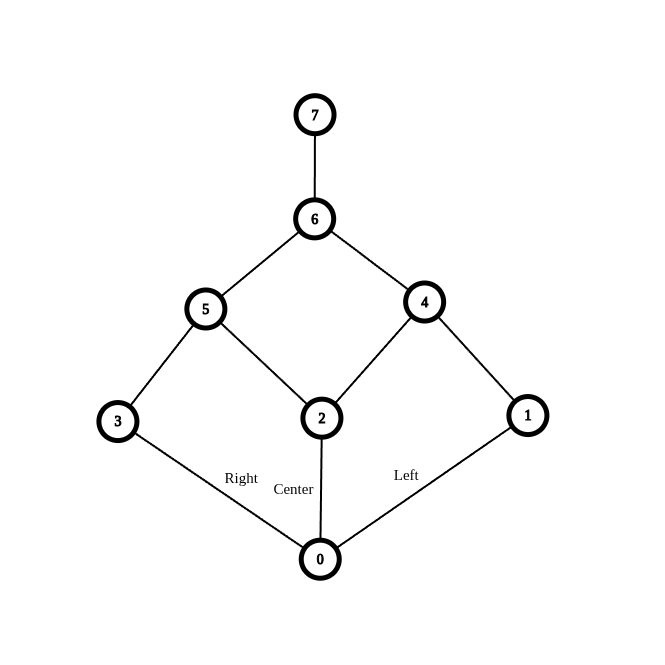
\includegraphics[width=\linewidth]{graph (1).png}\\
  \small (a)
\end{minipage}\hfill
\begin{minipage}{0.49\textwidth}
  \centering
  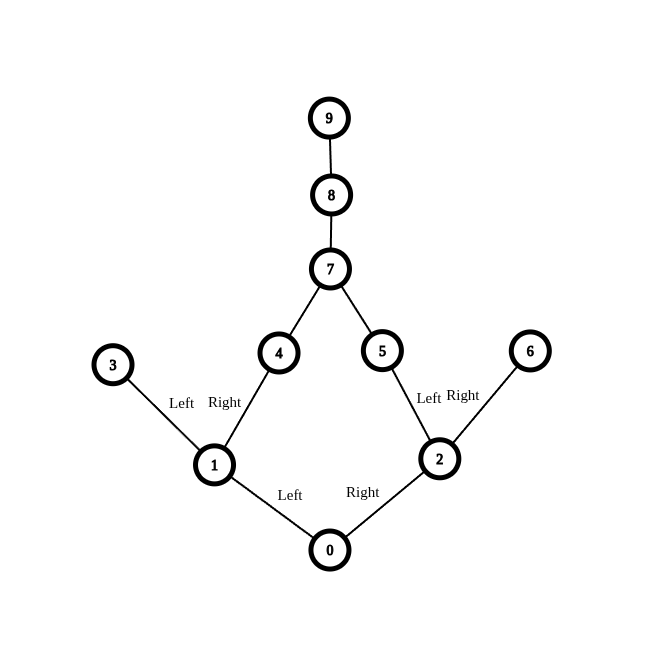
\includegraphics[width=\linewidth]{graph (2).png}\\
  \small (b)
\end{minipage}
\caption{Examples of object-support graphs generated by the VLM from target assembly images. Directed edges encode support relations that are later used for branch clustering and layer-based cutting.}
\label{fig:layered_graph}
\end{figure*}b

\begin{figure*}[!t]
\centering
\setlength{\tabcolsep}{2pt}
\begin{tabular}{ccc}
  
\includegraphics[width=0.32\textwidth]{fmb_1/001.png} &
  
\includegraphics[width=0.32\textwidth]{fmb_1/002.png} &
  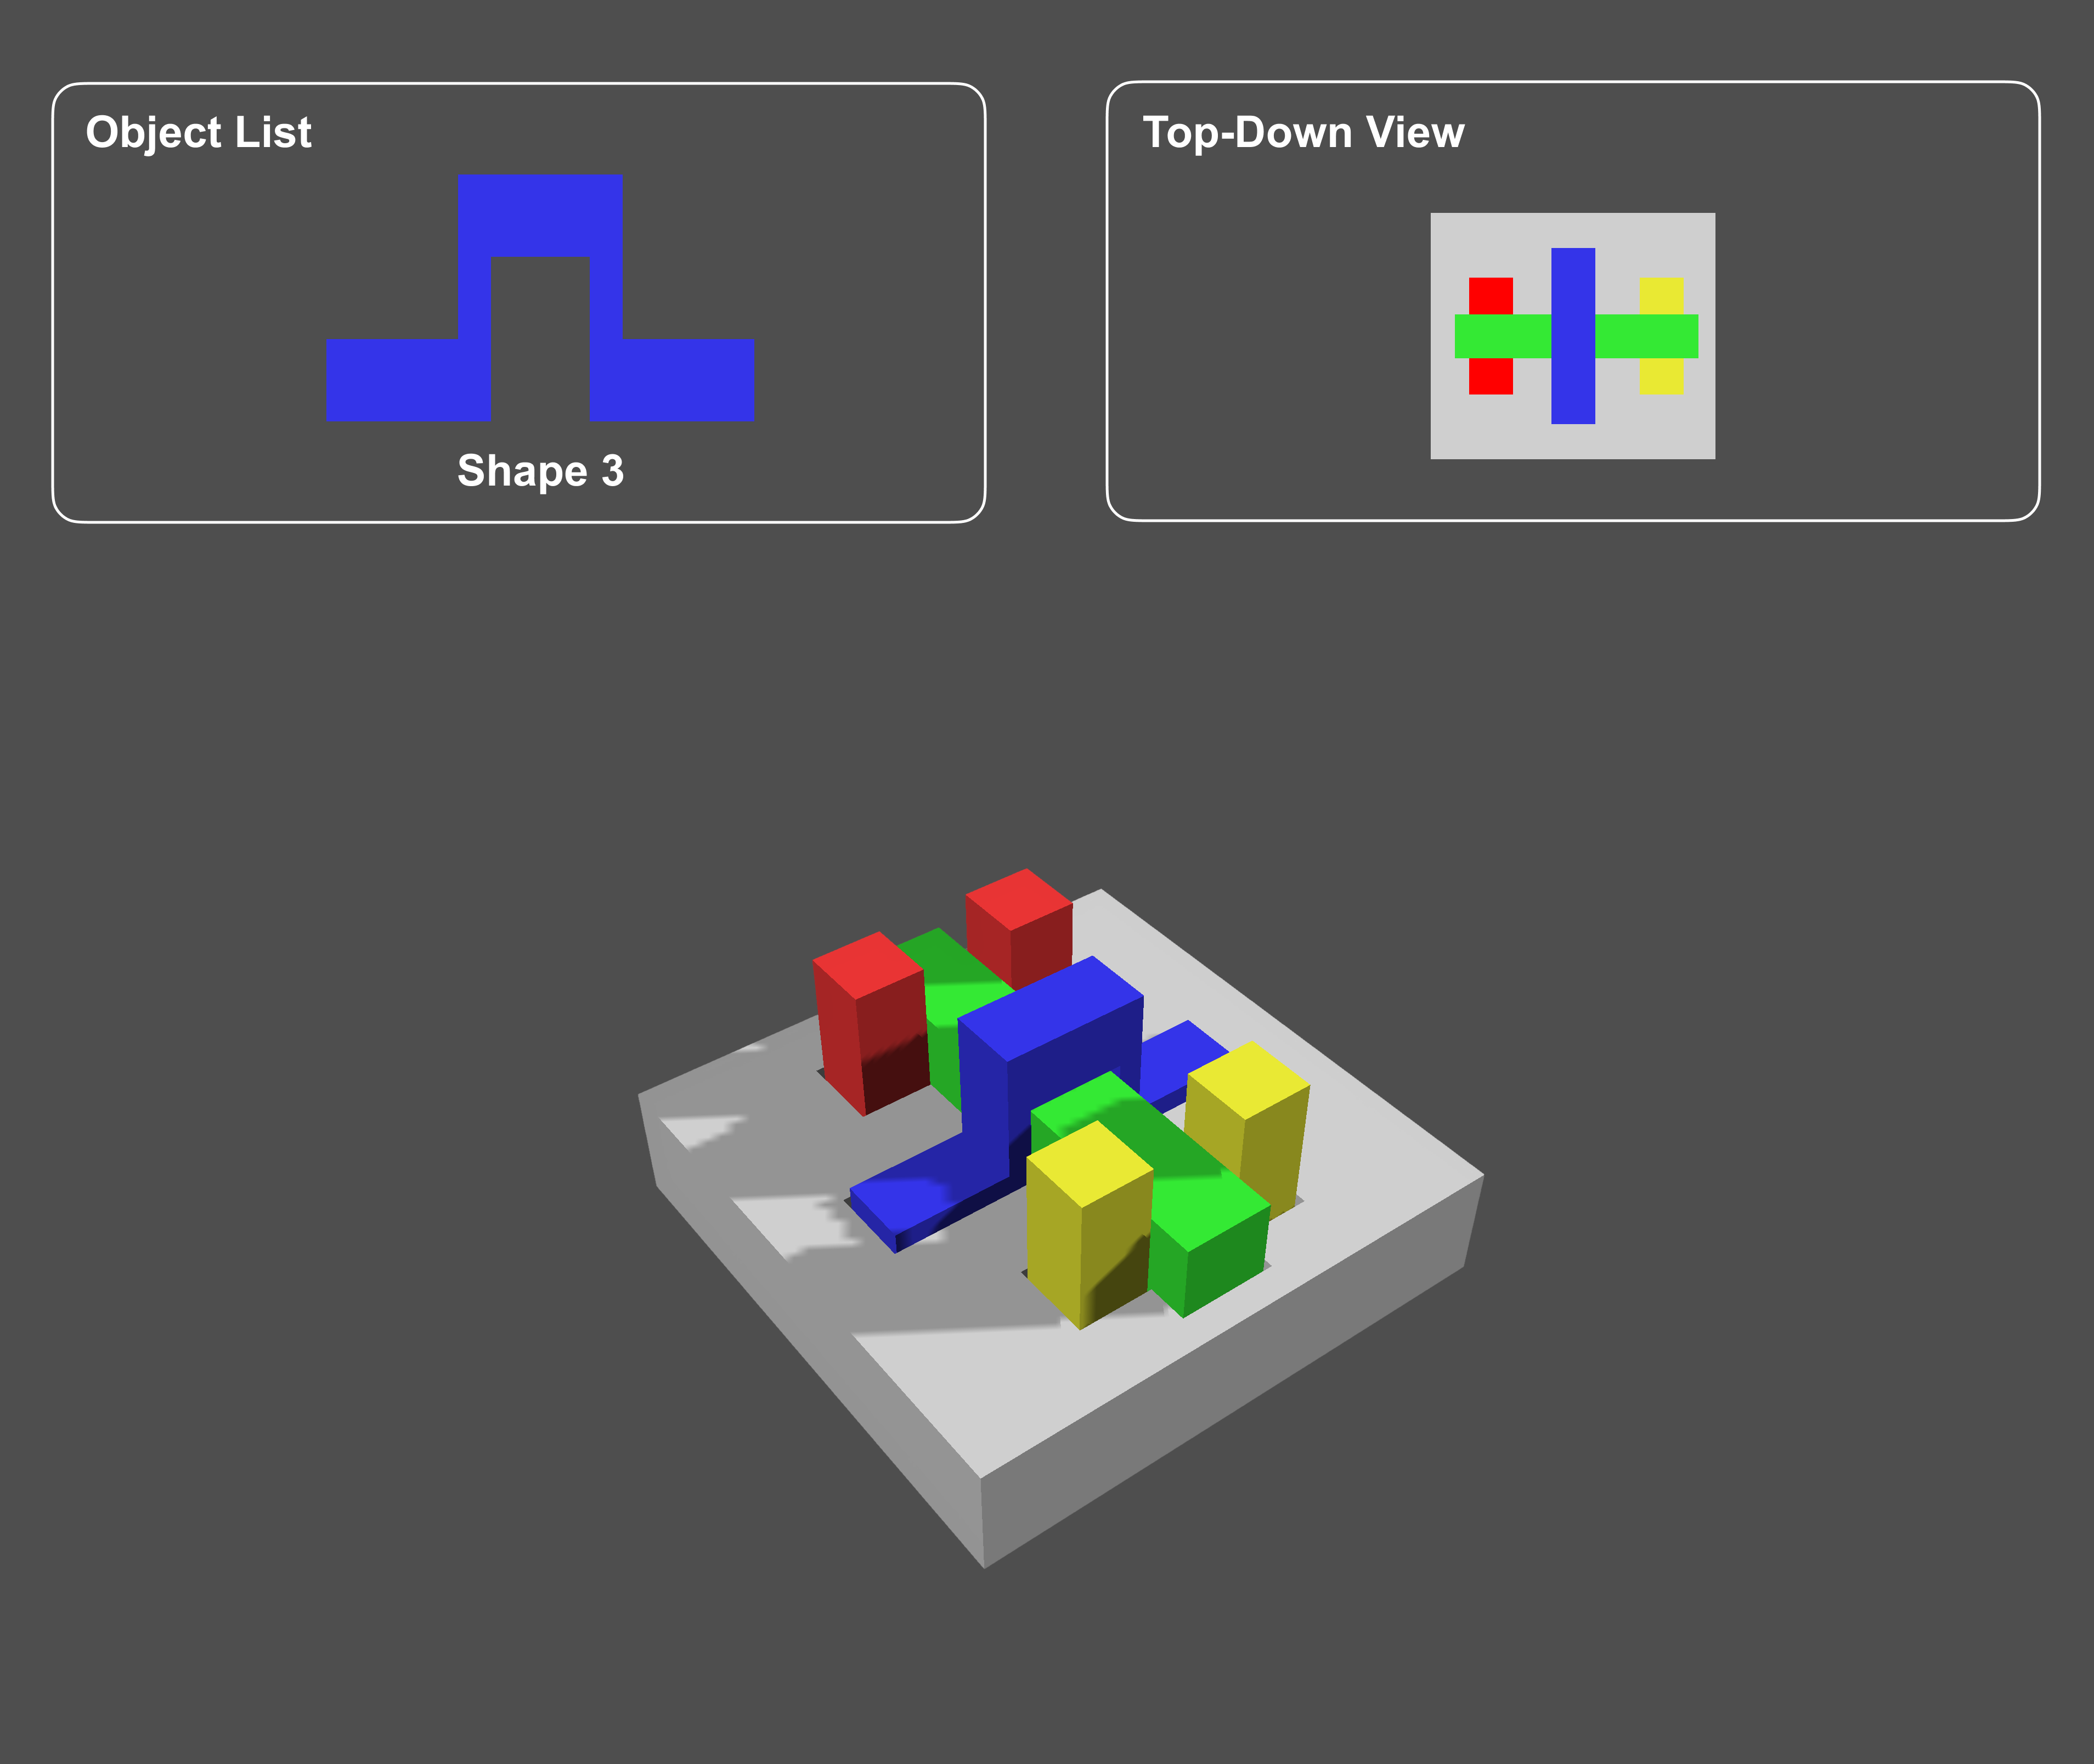
\includegraphics[width=0.32\textwidth]{fmb_1/003.png} \\
  \multicolumn{3}{c}{\small FMB-1 (left-to-right continuous sequence)}
\end{tabular}
\vspace{2mm}

\begin{tabular}{cc}
  
\includegraphics[width=0.48\textwidth]{fmb_3/001.png} &
  
\includegraphics[width=0.48\textwidth]{fmb_3/002.png} \\
  \multicolumn{2}{c}{\small FMB-3 (left-to-right continuous sequence)}
\end{tabular}
\caption{FMB visual examples arranged as left-to-right continuous strips for each folder.}
\label{fig:fmb_strips}
\end{figure*}

\subsection{Task Decomposition via Layer-Based Clustering}
\label{subsec:phase2}

Once the support graph is available, the next problem is to determine a concrete
execution order: which objects should be placed first, and which objects can be
placed together in a single solver call. Placing all objects simultaneously makes the
problem too large and computationally expensive, while placing objects one at a time
is unnecessarily slow. The decomposition must also respect the support constraint: an
object cannot be placed before all of its supporters are already in position.

We solve this with a layer-based clustering algorithm that operates directly on the
support graph in three steps.

\subsubsection{Step 1: Assign a Layer Number to Each Node}

The layer number of a node captures how many support steps it is away from the table.
The table root (node 0) is assigned layer~0. Every object resting directly on the
table has layer~1; an object resting on a layer-1 object has layer~2, and so on.
Formally:
\begin{equation}
  \mathrm{layer}(v) = 1 + \max_{u \in \mathrm{supporters}(v)} \mathrm{layer}(u),
  \label{eq:layer}
\end{equation}
where $\mathrm{supporters}(v)$ is the set of objects that directly support $v$.
This is computed iteratively until all nodes have a layer assignment. The layer
captures the minimal precedence requirement: a layer-$k$ object can only be placed
after all objects at layers $1$ through $k-1$ in its support chain are placed.

\subsubsection{Step 2: Group Nodes within Each Layer by Support Signature}

Within a given layer, objects that share the same set of direct supporters are
structurally siblings and can be placed consecutively. We therefore group objects by
their \emph{support signature}, defined as the sorted set of their direct supporter IDs
within the same branch:
\begin{equation}
  \mathrm{sig}(v) = \mathrm{sorted}\bigl(\mathrm{supporters}(v) \cap \mathcal{B}\bigr),
  \label{eq:signature}
\end{equation}
where $\mathcal{B}$ denotes the node set of the current branch.
Objects with the same signature form one group within that layer.
Bridge-structured objects, whose supporters span multiple branches, are assigned to
a dedicated bridge branch and handled separately.
Within each group, objects are ordered by their node identifier, which provides a
stable and deterministic execution order. Spatial annotations (left, center, right)
on the edges are used during branch assignment to distinguish parallel construction
sequences, but do not directly govern the intra-group ordering.

\subsubsection{Step 3: Build the Global Execution Order Iteratively}

Starting from the table, the algorithm collects the set of nodes whose supporters are
already placed (the \emph{ready set}), selects those at the lowest layer, groups them
by support signature, orders each group by node identifier, and splits each group into
execution batches of at most $B_{\max} = 2$ objects. The resulting batches are
appended to the global execution sequence, the placed nodes are recorded, and the
process repeats until all objects are scheduled.

For a nine-object assembly with three independent stacks (objects 1,3,4 on the left;
2,5,6 in the center; 7,8,9 on the right), this procedure produces the global
execution sequence $1 \mid 34 \mid 2 \mid 56 \mid 7 \mid 8 \mid 9$,
where the vertical bars separate execution batches submitted to the solver.

\subsection{Scene Grounding}
\label{subsec:scene_grounding}

Scene Grounding prepares the initial scene for downstream solving by identifying which
object instances remain executable and how they should be preferred when multiple
feasible candidates are available. It contains two complementary stages:
Reachability Screening removes infeasible objects, and Manipulability-Aware Ordering
ranks the reachable remainder.

\subsubsection{Stage 1a: Geometric Prior Scoring}
\label{subsec:gmm_esdf}

Before any solver is invoked, each object in the scene is assigned a scalar
reachability score approximating how accessible it is based on its position relative
to the surrounding scene geometry. The score combines two components.

The first is a density-based score computed with a Gaussian kernel of bandwidth
$\sigma = 0.12\,\mathrm{m}$ over all pick-candidate points in the scene:
\begin{equation}
  s_{\mathrm{gmm}}(o_i) = \frac{1}{N} \sum_{j=1}^{N}
    \exp\!\left(-\frac{\|p_i - p_j\|^2}{2\sigma^2}\right),
  \label{eq:gmm_score}
\end{equation}
where $p_i$ is the pick point of object $o_i$ (the handle sub-frame center if
available, otherwise the geometric center) and $p_j$ ranges over all $N$ candidate
pick points. A higher score indicates the object is located in a geometrically central
region of the workspace, which correlates with accessibility.

The second is a clearance score measuring distance from surrounding obstacles, each
approximated as a bounding sphere with center $c_k$ and radius $r_k$:
\begin{equation}
  s_{\mathrm{esdf}}(o_i) = \min_k \frac{\max\!\left(0,\ \min\!\left(\|p_i - c_k\| - r_k,\ d_{\max}\right)\right)}{d_{\max}},
  \label{eq:esdf_score}
\end{equation}
where $d_{\max} = 0.20\,\mathrm{m}$. A higher score indicates more open space around
the object.

The two scores are linearly combined:
\begin{equation}
  s(o_i) = \alpha \cdot s_{\mathrm{gmm}}(o_i) + \beta \cdot s_{\mathrm{esdf}}(o_i),
  \label{eq:reach_score}
\end{equation}
with $\alpha = 0.6$ and $\beta = 0.4$. An object is considered geometrically
accessible if $s(o_i) \geq \tau_r = 0.45$; otherwise it is flagged as infeasible.

\subsubsection{Stage 1b: Pick-Waypoint Feasibility Check}
\label{subsec:phase0}

Objects surviving Stage~1a are subjected to a kinematic feasibility check. For each
candidate $o_i$, we construct a single-step KOMO subproblem that asks the solver
to find a robot configuration from which a grasp of $o_i$ can be initiated. The
subproblem uses the same KOMO/RAI framework as the main solver and includes the full
set of kinematic and collision constraints; FCL and libccd serve as the collision
detection backend of the RAI library. An object is declared reachable if and only if
this subproblem is feasible:
\begin{equation}
  \mathrm{Reach}(o_i) =
  \mathbb{I}\!\left[\mathrm{Feasible}\!\left(\Pi_i^{\mathrm{pick}}(o_i)\right)\right],
  \label{eq:reachability}
\end{equation}
where $\Pi_i^{\mathrm{pick}}$ is the pick-waypoint subproblem for object $o_i$.
An object is marked infeasible if either Stage~1a or Stage~1b flags it; only objects
passing both stages are retained for downstream use. The two-stage structure is
intentional: the geometric prior stage filters obviously unreachable objects cheaply,
while the pick-waypoint check provides rigorous kinematic verification at low cost.

\begin{figure}[!ht]
\centering

\includegraphics[width=\columnwidth]{Reachability.png}
\caption{Reachability screening result: objects passing both the geometric prior and the pick-waypoint feasibility check are retained (reachable), while the remaining candidates are pruned before downstream LGP solving.}
\label{fig:reachability}
\end{figure}

\subsubsection{Manipulability-Aware Ordering}
\label{subsec:phase0_manip}

After reachability screening, the surviving objects are ranked by how comfortably the
robot arm can approach them. For each reachable object $o_i$, we define an approach
target slightly above the object, solve a damped least-squares inverse kinematics
problem for that target, and evaluate the positional Yoshikawa manipulability score:
\begin{equation}
  m(o_i) = \sqrt{\det\!\left(J_p(q_i)J_p(q_i)^\top\right)},
  \label{eq:manipulability}
\end{equation}
where $J_p(q_i)$ is the position Jacobian of the robot at the IK solution $q_i$.
Objects with a higher manipulability score are ranked earlier in the candidate list
for their object type. Objects for which the IK fails are placed at the end of the
list. This ranking is later used in the execution-order embedding stage to select
which physical object instance should be used when the task decomposition calls for
an object of a given type.

\begin{figure}[!ht]
\centering
\setlength{\tabcolsep}{2pt}
\begin{tabular}{cc}
  
\includegraphics[width=0.48\columnwidth]{Manipulability_1.png} &
  
\includegraphics[width=0.48\columnwidth]{Manipulability_2.png} \\
  
\includegraphics[width=0.48\columnwidth]{Manipulability_3.png} &
  
\includegraphics[width=0.48\columnwidth]{Manipulability_4.png}
\end{tabular}
\caption{Manipulability scores evaluated for four candidate object instances. Higher scores indicate more dexterous approach configurations; instances are ranked accordingly to guide scene-side grounding.}
\label{fig:manipulability}
\end{figure}

\subsection{Execution-Order Embedding}
\label{subsec:phase_embed}

At this stage, the two parallel streams are merged. Task Decomposition has produced a
global execution sequence of batches, where each batch specifies a set of structural
slots to be filled (e.g., ``place a box-type object on top of cube\_1''). Scene
Grounding has produced, for each object category, a ranked list of concrete scene
instances that are both reachable and ordered by manipulability.

Execution-Order Embedding binds each structural slot in the current batch to a
concrete scene instance by iterating down the ranked candidate list for the
corresponding object type until a match is found. The output is a fully grounded
batch specification: a list of concrete object-to-role assignments that can be handed
directly to the LGP solver.


\subsection{Selective LGP Solving with Active Constraints}
\label{subsec:phase3}

Native LGP couples symbolic task structure with continuous trajectory
optimization through a shared representation of predicates, action semantics,
and decision rules~\cite{cite_lgp_2015}. In principle, this abstraction can
solve assembly tasks from symbolic goals alone. In long-horizon settings,
however, directly exposing the full generic task domain still leads to
excessive symbolic branching and unnecessary geometric backtracking.

Our solver therefore instantiates the native LGP abstraction selectively for
each grounded execution batch. For the current batch, it compiles only the
symbolic relations, object bindings, and decision rules required by the active
support pattern. The solver thus receives a grounded symbolic-geometric
subproblem tailored to the current batch rather than a monolithic domain
covering all possible assembly alternatives.

In our problem formulation, a trajectory is discretised as $\mathbf{x}_{0:T} = \{x_0, x_1, \dots,x_T\}$.
We first keep the native LGP formulation in its original joint form~\cite{cite_lgp_2015}
\begin{align}
\min_{\substack{x,\,a_{1:K},\\ s_{1:K},\,t_{1:K}}}\quad
&\int_0^T c\!\left(x(t),\dot{x}(t),\ddot{x}(t)\right)\,dt + \psi\!\left(x(T)\right)
\label{eq:lgp_joint_objective}\\
\text{s.t.}\quad
&\forall k=1{:}K\ \ s_k = \mathrm{succ}(a_k, s_{k-1}),
\label{eq:lgp_logic_transition}\\
&s_K\models g,
\label{eq:lgp_goal_constraint}\\
&\forall_{k=1}^{K}\ h_{\mathrm{switch}}\!\left(x(t_k)\mid a_k,s_{k-1}\right)=0,
\label{eq:lgp_switch_constraints_eq}\\
&\forall_{k=1}^{K}\ g_{\mathrm{switch}}\!\left(x(t_k)\mid a_k,s_{k-1}\right)\le 0,
\label{eq:lgp_switch_constraints_ineq}\\
&\forall t\in[0,T]\ h_{\mathrm{path}}\!\left(x(t),\dot{x}(t)\mid s_{k(t)}\right)=0,
\label{eq:lgp_path_constraints_eq}\\
&\forall t\in[0,T]\ g_{\mathrm{path}}\!\left(x(t),\dot{x}(t)\mid s_{k(t)}\right)\le 0.
\label{eq:lgp_path_constraints_ineq}
\end{align}

For each grounded batch, we then solve the corresponding $k$-order Markov Optimization (KOMO) subproblem in
its original constrained sum-of-squares form~\cite{cite_komo_2014}, i.e., the continuous trajectory-optimization component of LGP, to compute robot and object motions subject to kinematic, task, and collision constraints.
\begin{align}
\min_{x_{0:T}}\quad
&\sum_{t=0}^{T} f_t\!\left(x_{t-k:t}\right)^\top f_t\!\left(x_{t-k:t}\right)
+\sum_{t,t'} k(t,t')\,x_t^\top x_{t'}
\label{eq:komo_batch}\\
\text{s.t.}\quad
&\forall t:\ g_t\!\left(x_{t-k:t}\right)\le 0,\ h_t\!\left(x_{t-k:t}\right)=0.
\label{eq:komo_batch_constraints}
\end{align}

The same waypoint-level solve also provides geometric cues for downstream
motion optimization. Let $x$ denote the full-motion trajectory optimized in
the downstream stage, let $d_{ij}(x)$ denote the minimum pairwise distance
between collision proxy frames $f_i$ and $f_j$ along $x$, and let $f_i^w$ denote
the pose of frame $f_i$ at waypoint $w$. The downstream trajectory is obtained
by solving
\begin{equation}
x^* = \arg\min_x J(x),
\label{eq:active_objective}
\end{equation}
subject to collision constraints instantiated only for the active set
\begin{equation}
c_{ij}(x) = d_{\mathrm{safe}} - d_{ij}(x) \leq 0,
\quad \forall (f_i, f_j) \in \mathcal{C}_{\mathrm{active}}(w),
\label{eq:active_constraints}
\end{equation}
where
\begin{equation}
\mathcal{C}_{\mathrm{active}}(w) =
\left\{(f_i, f_j)\ \middle|\ d(f_i^w, f_j^w) < r_{\mathrm{active}}\right\}.
\label{eq:active_set}
\end{equation}
Here, $J(x)$ denotes the downstream motion objective, $d_{\mathrm{safe}}$ is
the prescribed safety margin, and $r_{\mathrm{active}}$ is the activation
radius used to screen candidate collision pairs from waypoint geometry.
Only pairs selected by $\mathcal{C}_{\mathrm{active}}(w)$ are instantiated
as explicit collision constraints in the downstream full-motion solve. This
active-constraint strategy reduces unnecessary collision checks and shortens
full-motion solve time without altering the structural plan itself.

This restricted instantiation preserves the expressiveness of native LGP while
concentrating the search on the structurally relevant portion of the task. It
also provides a clean interface between graph-level decomposition and
geometric solving: the decomposition module decides which support relations should be
realized next, and native LGP resolves whether and how those relations can be
executed under the current scene geometry.

\subsection{Real Robot Execution}
\label{subsec:phase4}

After each subproblem is solved, the resulting trajectory is parsed and
dispatched to the robot controller for execution on the physical platform.
The execution layer remains intentionally thin: it reads the planned motion
and gripper commands, executes them on the real robot, and updates the scene
state for the next planning-solving cycle.

\begin{figure}[!t]
\centering
\includesvg[width=\linewidth]{accuracy_bar_chart}
\caption{FMB VLM accuracy summary (from extracted FINAL\_JSON blocks).}
\label{fig:fmb_accuracy}
\end{figure}





\bibliographystyle{IEEEtran}
\bibliography{ref.bib}

\end{document}
